\chapter{Background}

In this chapter, we will look at the fundamental concepts and background information needed to understand the the different infections model, problem with seed-selection for social networks, and solving Breadth-first search using matrix multiplication. This chapter will contain notations that we would use throughout the report and used in the field. One aspect we will focus focus on, is how we can performe graph algorithm such as breathd irst search as matrix multiplication.


\section{Network terminology and glossary}
The fundamental unit in a network is $\it{{Vertex}} (pl. vertices)$ sometimes called a node (computer science). For this report, vertex and node would be used intergangably. The "bridge" or the line connectiong two vertices is called a $\it{{Edge}}$, wich serves as a connection between verices as shown in Figure \ref{fig:SimpleGraph}.  Different network have different types of edge, some can be $\it{Directed}$ or $\it{undirected}$. Directed edge is where a edge  runs in only one direction (such as a one-way road between two points), and undirected if it runs in both directions. Directed edges, which are sometimes called arcs, can be thought of as sporting arrows indicating their orientation. A graph is directed if all of its edges are directed. An undirected graph can be represented by a directed one having two edges between each pair of connected vertices, one in each direction.

\begin{figure}[!ht]
	\caption{Simple network} 
	\label{fig:SimpleGraph}
	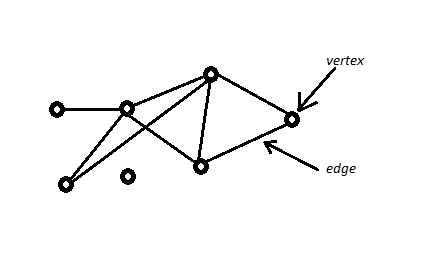
\includegraphics{smallExampleNetwork}
\end{figure}


Each node have a value that is known as $\it{{Degree}}$. Degree for a node is the number of edges connected to a vertex. Note that the degree is not necessarily equal to the number of vertices adjacent to a vertex, since there may be more than one edge between any two vertices. In a few recent articles, the degree is referred to as the “connectivity” of a vertex, but we avoid this usage because the word connectivity already has another meaning in graph theory. A directed graph has both an in-degree and an out-degree for each vertex, which are the numbers of in-coming and out-going edges respectively. The $\it{{Component}}$ to which a vertex belongs is that set of vertices that can be reached from it by paths running along edges of the graph. In a directed graph a vertex has both an in-component and an out-component, which are the sets of vertices from which the vertex can be reached and which can be reached from it.

A $\it{{Geodesic path}}$ is the shortest path through the network from one vertex to another. Note that there may be and often is more than one geodesic path between two vertices. The $\it{{Diameter}}$ of a network, however,  is the length (in number of edges) of the longest geodesic path between any two vertices. A few authors have also used this term to mean the average geodesic distance in a graph, although strictly the two quantities are quite distinct

\section{Network}
A $\it{network}$ is a collection of $\it{Vertices}$, commonly known as nodes with $\it{edges}$ connecting them together\cite{ComplexNetwork2003}. The edges serves as a connection, or a "bridge" between the nodes, while the nodes can reprecent something, or containing information. In the real world, multiple systems takes the form of networks around the world, examples are the internettt, the World Wide Web, social media like Facebook, twitter etc.  There are different types of network or $\it{graphs}$. These include from $\it{social network}$, $\it {sinformation networks}$, $\it{technological networks}$ ,and $\it{biological network}$.  Each of them have a different properties, but we will focus more about social network.

A social network is a set of people connected to each other via some form of contact or interactions\cite{ComplexNetwork2003}. The nodes are people while the edges are the connections between peoples. The social network display information regarding connection, interaction or location of a set of people.It forms patterns regarding friendships, business interactions between companies and families history/ ancestral tree. The social network is often used in social science\cite{ComplexNetwork2003}. Some noteable experiments are \cite{smallWorldExperiment}, which looks at the small world problem. The small world problem can be summarized as: "what is the probability that any two people, selected arbitrarily from a large population, such as that of the United States, will know each other?". \cite{smallworldExperiment1969}. This in itselfe is not that interesting, the \cite{SmallworldExperiment1969} takes that altho person $\it{a}$ and $\it{z}$ does not know each other, do they have a set of individuals \{ $\it {b_1, b_2, ... b_n} $\} who are mutual friend or even a "chain" of such individual($\it {a-b-c-...-y.z}$).

Some properties that networks often exhibits are the small world effect, transitivity or clustering, degree correlations, and community structure\cite{ComplexNetwork2003}. Different networks would have some of the specific properties and values. Social network would have a small world effect of around 6 degree, with high transitivity and have a community structure, while a information network, such as a citation network, would most likely have high transitivity since citation and publication have different publication date. Paper A refers to Paper B, which refers to paper C, but paper C can not possibly refer to papaer A since C is clearly published before paper A. [INSErt fIGUre.]

\subsection{The small world effect}
The small world effect was first demonstrated by Stanley Milgra in the 1960s during his famous letter passing experiment\cite{SmallWorldProblemSmilgram1960}. The experiment was about passing letters from person to person to reach a designated target with only small steps. For the published case, the chain was around six \cite{Experiment1969}. This shows us that for most pair of vertices in a network can reach each other with a short parth. A more precise wording is that "Networks are said to show the small world effect if the value of $\it{l}$ scales logarithmically or slower with the network size for a fixed mean degree.". \cite{ComplexNetwork2003}. We have defined $\it{l} $ to be the mean geodesic distance between vertex pairs in a network.

For the information diffusion problem, this kind of effect would result in that the  iffusion through a network would need around 6 steps to have traveled through the entire network. Meanning that most node can reach each other through a relatively small step.

\subsection{Transistivity/clustering}
Transistivity, also sometimes called clustering is the properties that shows that there is a high number of triangles in the network. A triangle in a network is if node A is connected to node B and node C, and node B and C is also connected to each other, thus creating a triangle. In social network, we say that a friend of your friend is likely to be your friend too\cite{ComplexNetwork2003}. The transistivity is often used to show $\it{network density}$.

For information diffusion and seed selection, this would mean that picking nodes that are geographically close/neighbour to each other, would have a smaller impact/spread then picking two not neighbouring vertecies. By picking two nodes that are connected to each other, they would likely share a common neighbour thus having a limited reach.  

\subsection{Degree distribution}
Degree distribution is the histogram of degrees of vertex. For random graphs, the distribution would most likely be a poiison distribution or binomial. For real world network, the distribution would often have a highly rightskewed distribution. Resulting in that the distribution has a long right tail of values. The probability $P_k$ is the probability that the new vertex $\it{v}$ have the degree k. 

The degree distribution shows us how the degree to the graph is distributed. For social graph, the degree distribution is often in the shap of [INSERT FOIGURE of degree distribution histogram]. For the information diffusion, this distributon shows us how many high degree nodes there are in the network, those node would likely be high prioritized node and have a large impact. 

\subsection{Degree corrrelations}
As [REFER TO FIGURE OF DEGREE DISTRIBUTION] show, the network have a degree distribution with few high degree nodes and multiple low degree nodes. One interesting properties is the degree correlations. Degree correlations is how the high degree and low degree nodes connects to each other. One question is if high degree nodes tends to connect to other high degree nodes, or do they prefer to connect to low degree nodes. It turns out that both incidents is found in networks\cite{complexNetwork}. We can see that for all social network measured in \cite{complexNetwork}, the social networks are assortative, meaning vertices have a selective linking, where high degree vertex connects to other high degree vertex\cite{AssortativeMixing2002} 

For data diffusion, this kind of behaviour would result in wasting a seed by picking majority of high degree node for starting seed, since most of them would be connected to each other. One solution is by mixing the selection, choose some percentage to be high degree, and some with lower degree.


\subsection{Network resilience}
For most network model, there is the need to remove nodes from the network. Removal of a node can have no effect on the network as a whole, or it can be devastating. Network resilience looks at how the network can ressist to such a removal. There are two different removal scheme, the random removal where nodes are randomly picked and removed, or the targeted removal where specific nodes are removed depending on the critteria. 

The experiment mentioned in \cite{complexNetwork} by Albert $\it{et al}$ showed that for a subset of network representing the internett and the world wide web, targeted removal had a larger impact then random removal. The targeted removal removed the highest degree nodes from the network, and the random removal removed nodes randomly. The random removal had a minimal effect on the network, while the targeted removal had a much larger impact, the mean vertex-vertex distance increased. They proposed that the internett was highly resilient to random removal, while much more vuarneble to targeted removal. 

There are other studies that proposed a different interpetation about the data found.	

In an example of information diffusion, a targeted removal would result in massive change to the diffusion path. By removing high degree node would result in remove influential nodes and limit the spread of the data. Removing important node connection two different communitys would result in isolation and no path towards other community.

\subsection{community structure}
One properties that is often observed in a social network, is the community structure. The community structure is where a group of vertecies having high density of edges with each other, while having lowe density of edges to other "community". We can see an example of the community structure clearly displayed from \cite{RaceSchool2001}. Where we can see the playground was divided into different community.

This type of community structure would have a lagre impact on how the algorithm would select a seed for information diffusion. If all the seed would be selected in one community, the probability of spreading over to other community would be smaller, them having a seed be in the other community.

\section{Matrix notations}
By using a linear algebraic approach to solve graph algorithms often gives us a variety of benefit include easier implementation, higher preformance and syntactic simplicity. \cite{MathToAlgo}. There are multiple reasons to do graph algorithms as linear algebra. This can show potentially improvement, potentially optimization and be more visually clear how the algorithm is. 


\subsection{Semiring}
A $semiring$ is a set of elements with two binary operations. The two operations are often known as "addition" and "multiplication". By this definition, [SYMBOL FOR BOOLEAN] and [SYMBOL FOR INTEGER]. are both semirings.  One way to performe graph algorithm, is apply matrix multiplication over such semirings. One of the common notation in writing the semiring, is $a+b$ and $a \ast b$. This can be confusin, so often there will be some special semiring operator.

\subsection{Sparce Matrix}
A sparce matrix is an matrix with few non-zero elements in them. The social network can often be reprecented with a sparce matrix. An sparce matrix have its majority of element as zero, as shown in fig{INSERT FIGURE OF SPARCE MATRIX}. We can represent a social graph in the form of a sparse matrix. In an adjacency matrix, a cell containing 1 means a connection is presence, while a 0 is lack no connection. So, as we can see in the Figure \ref{fig:adjacencyM}, as we can see at coordinate $[1,3] = 1$. This tells us that there is a edge between vertex 1 and vertex 3. The adjacency matrix is commonly used to represent an graph such as Figure \ref{fig:AdjacencyM} and Figure \ref{fig:matrix}.

\begin{figure}
	\begin{subfigure}{0.5\textwidth}
	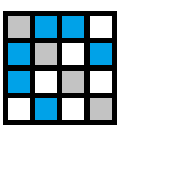
\includegraphics{AdjacencyM}
	\caption{The ajacency matrix}
	\label{fig:AdjacencyM}
	\end{subfigure}


	\begin{subfigure}{0.5\textwidth}
	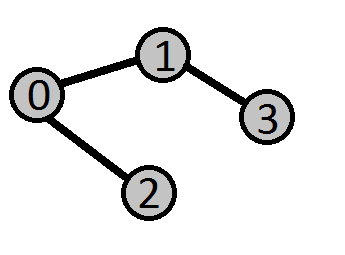
\includegraphics{simpleGraph}
	\caption{The graph corresponding to the adjacency matrix}
	\label{fig:matrix}
	\end{subfigure}
	 	
\end{figure}

\section{Data diffusion}
Data diffusion is looking at how information is propagated through a network or a graph. An example would be how a new Internet meme, a new trend or how a new disease is spread through a community. The process consist of a set of starter nodes that are "infected", during each time-step, there are a chance that the "infected" node would "infect" its neighbor. To start such a simulation, we would need to first pick out a set of initial "starter node". These {\it k} seed nodes is a set of node that in the initial time-step is infected. They will pass on the information/infection during each time-step and the information/infection will propagate through the network.

\section{Basic Diffusion Models}
When we talk about information propagation, we can look at how diseas or technological innovations is spread through a social network. We can simulate those kind of behavior with different diffusion models. There are two basic diffusion models used to simulate the propagation of information through a network\cite{MaximizeSpread2003}, the {$\it linear threshold model$} and the $\it{ independent cascade model}$\cite{MaximizeSpread2003}.

This process can be simulated by looking at a social network and how information propagates through the network. We look at each node in the graph as a person, they can be either active, or inactive. The activation of a node depends on which diffusion model we choose. A active node is "infected", while the inactive is the "healthy" ones. The activation of each nodes is dependent on which model we pick.

The linear threshold model uses a threshold $\theta_v$ between the interval [0,1], which represent the faction of $\it{v}'s$ neighbors that need to be active to activate node $\it{v}$. The Linear Threshold Model activates the current node {\it v} when the weight ${\it b_{v,w}} > \theta$ from its neighbor $\it{w}$ outweighs the $\theta_v$. This is more in line with the situation were each person have a chance to adopt to a new trend if exposed to the trend enough time by his close friends. An example would be a product promoted on social network like twitter and Facebook. The user will adopt the new trend if he is exposed to it from enough friends or idols. As show in Figure \ref{fig:linearThresh}, the threshold for vertex $\it{v}$ to be activated is $\theta_v$, a percentage of the total neighbour, in this instance, three.

\begin{figure}[!ht]
	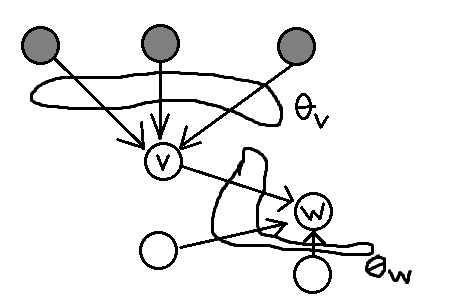
\includegraphics{linearThreshold}
	\caption{Linear Threshold model} 
	\label{fig:linearThresh}
\end{figure

The independent cascade model changes states with a probability $\it{p_{v, w}}$, where $\it{ v }$ is current node, and $\it{w}$ is it's neighbor. During each propagation, the node $\it{v}$ have a  $\it{p_{v, w}}$ chance to change state if the neighbor $\it{w}$ changed state. If during time-step $\it{t}$ a node $\it{v}$ changed state, its neighbor $\it{w}$ would have a $\it{p_{v, w}}$ chance to change state in the next time step. An example here would be spread of a disease. The current node$\it{v}$ have a chance($\theta_v$) to activate its neighbor. As shown in Figure \ref{fig:ICM}, there is an probability of $p_v$ to infect the neighbours to vertex v, in this figure, the probability is the same, bit that is not nessesary true. the probability can be independent, each vertex can have different probability to activate neighbour, or we can have a global probability.

\begin{figure}[!ht]
	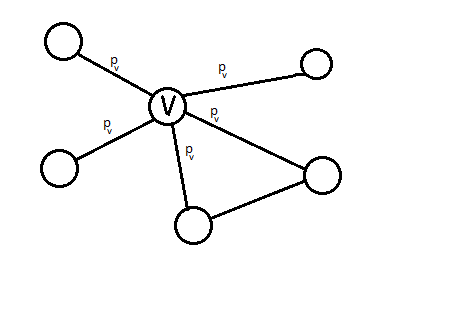
\includegraphics{ICM}
	\caption{Independent cascate model} 
	\label{fig:ICM}
\end{figure

We can se the similarity between the breadth first search and information diffusion. Breath first search, as mentioned before, starts at the root node and add the root nodes children in a queue, then tales the first childe node in the queue and adds all its childen to the queue. Each new child node is added to the back of the queue, while finished node is placed in a $\it{finished_queue}$. The sequences of nodes tested is the same as during an information diffusion, where the diffusions neighbour is placed in the $ \it{boarder_queue} $ and having a probability to be infected. If the node is infected, then that nodes neighbour would be added to the $boarder_queue$, while if the node is not infected, the neighbour to the node would be safe. The information diffusion can therefore be looked at as an breadth first search, with an probability to add the child to the queue. 

\section{Breadth First Search as a matrix multiplication.}
By looking at the connectivity matrix, we can see that a connectivity matrix is a graph represented in a matrix format. The BFS can be achieved by looking at the BFS operations as a matrix multiplication \cite{algoToMath}. If we look at the graph as a connectivity matrix, we can apply matrix multiplication to generate the breadth first search. 

Breadth first search is an tree traversal algorithm. BFS start at the root node $\it{r}$, or any arbitary node in a n tree, and stores all its child node in an $\it{queue}$. The algorithm then takes the first node from the queue, $\it{v_1}$ and stores all the child node to $\it{v_1}$ in the back of the queue, this process continous until the queue is empty and all the nodes have been iterated over. From the psaudocode we can see:

\begin{algorithm}
\caption{Breadth First Search}
\begin{algorithmic}[1]
\State{$dist[\forall \it{v} \in V] = -1; currentQ, nextQ = \oldemptyset$}
\State $step = 0; dist[root] = step$
\State ENQUEUE(nextQ,root)
\While {$nextQ\neq \oldemptyset $}
\State $currentQ = newxtQ; nextQ = \oldemptyset$
\State $step = step+1$
\While {$currentQ \neq \oldemptyset$}
\State$ u$ = DEQUEUE(currentQ)
\For {$v \in Adj[u]$}
\If {$dist[v] == -1 $}
\State $dist[v] = step$
\State ENQUEUE(nextQ, v)
\EndIf
\EndFor
\EndWhile
\EndWhile
\Return dist
\end{algorithmic}
\end{algorithm}

We can also look at how an breadth first seaerch can be executed by appllying  sparce matrix multiplication. We can see that teh adjacency matrix is an sparse matrix. We can use sparce matrix umltiplpication to do graph algorithm, one example is the BFS. 


\section{BFS to data diffuison}
We can draw an distinctive line between the breadth first search and data diffusion. The breadth first search adds all the childe node from the parent node to a queue, then change the current node to the first node in the queue and repeats until the entire graph is iterated over, or the queue is empty. This is in teorie the same as data diffusion, where information is passed to the connected vertex. The new "infected node" can then pass on the information along to the other nodes that are connected to the new node and so on. This is in practice, the same as breadth first search, minus the searching part. 

We can in then draw teh conclution that Independent cascade model, is a modified version of the breadth first search, where each child note have a specific percent to be infected. The itteration is the same as a breadth first approach, but the result of the addition of node is dependent on a random "coin-toss".


\section{greedy algorithm}
The  greedy algorithm was proposed by Kempe \cite{MaximizeSpread2015}. The algorithm is a greedy algorithm where it finds the starter set of nodes $\it{S}$ by iterating through all the vertex in $\it{V}$ and calculate the total amount of spread. The spread is saved and the $\it{k}$ most influential nodes would be choosen.

 \begin{algorithm}
\caption{Greedy Algorithm}
\begin{algorithmic}[1]
\State Start with $A = \oldemptyset$
\While{$|A| \leq l$}
\State For each node $x$, use repeated sampling to approximate $\sigma(A \cup {x}) $ to within ($1 \pm \varepsilon$) with probability
$1 − \delta$
\State Add the node with largest estimate for $\sigma(A \cup {x})$ to A.
\EndWhile
\State Outpu the set $A$ of nodes.
\end{algorithmic}
\end{algorithm}

-degree algorithm

Another popular algorithm is the degree algorithm\cite{MaximizeSpread2015}. Unlike the greedy algorithm, the degree sort all the node acoring to their degree distribution. The algorithm picks the top $\it{k}$ nodes according to the degree distribution. This approach does not take the degree correalation into acount, by picking only high degree node, there would be multiple overlapping activated node.


Random algorithm
The last one is the random algorithm. The random algorithm just pick a random seed node. This approach is the simplest to implement and easiest. The downside is that this is random and there are no strategical choosing of seed node. 


\section{Cache oblivious model} 
A cache oblivious model ignores the cache size and line and designs the algorithm to be cross platform and optimized. An algorithm is $\it{cache aware}$ if it contains parameter that can be tuned to optimize the cache complexiity for the cache size\cite{CacheObli1999}. Such algorithm have the disadvantage where a adaptation is neede for a new architecture\cite{COmultiplic2009}. The cache oblivious model is designed for two level of memory, and assumes that tsuch an optimization is optimized for multiple levels as well. There are multiple algorithm designed that shows that such a model actually improves the algorithm. One of such is an cache oblivious sparce matrix multiplication. Sparse matrix multiplication is notorious to be inefficeint use of the cache system, it forces the user to jump throgh data in main memory\cite{COmuliplic2009}. The sparce matrix approach proposed \cite{COmultiplic2009} focus on reordering the matrix and row in an cache oblivious maner. There are results that shows that a cache oblivious approach have given improvement to computation time for some matrices during sparse matrixc multiplication, but for cache-friendly structure, this is shown to be a minor imporvement and even small loss. 